\documentclass[11pt, letterpaper]{article}

% --- 1. MODERN PREAMBLE ---

% Fonts and Encoding
\usepackage[utf8]{inputenc}
\usepackage[T1]{fontenc}
\usepackage{mathpazo} % Palatino font (serious, academic look)
\usepackage[scaled=0.95]{helvet} % Helvetica for sans-serif headers
\usepackage{microtype} % Improves text justification

% Layout and Geometry
\usepackage[margin=1in]{geometry}
\usepackage{parskip} % Block paragraphs (cleaner for reports than indentation)
\usepackage{setspace}
\setstretch{1.15} % Slightly more open line spacing

\usepackage{tikz}
\usetikzlibrary{intersections, arrows.meta, shadows} % Added 'shadows'

\usepackage{listings}
\lstdefinelanguage{yaml}{
  keywords={true,false,null,y,n},
  keywordstyle=\color{techblue}\bfseries,
  basicstyle=\ttfamily\footnotesize,
  breaklines=true,
  frame=single,
  rulecolor=\color{techgray},
  backgroundcolor=\color{white},
  stringstyle=\color{accentred},
  commentstyle=\color{gray}
}

% Colors and Links
\usepackage[table]{xcolor}
\definecolor{techblue}{RGB}{0, 50, 100} % Deep Navy
\definecolor{techgray}{RGB}{240, 240, 245} % Very light gray for boxes
\definecolor{accentred}{RGB}{180, 0, 0}

\usepackage[colorlinks=true, linkcolor=techblue, citecolor=techblue, urlcolor=techblue]{hyperref}

% Headers and Footers
\usepackage{fancyhdr}
\pagestyle{fancy}
\fancyhf{}
\lhead{\sffamily \footnotesize Refining MRV with UEVF}
\rhead{\sffamily \footnotesize ID TP-003}
\cfoot{\thepage}
\renewcommand{\headrulewidth}{0.5pt}


% Fix fancyhdr headheight warning
\setlength{\headheight}{14.5pt}
% Math and Theorems
\usepackage{amsmath, amssymb, amsthm}
\usepackage{bm} % Bold math

% Fancy Boxes for Propositions/Lemmas
\usepackage[most]{tcolorbox}
\newtcbtheorem[auto counter, number within=section]{proposition}{Proposition}{
  enhanced,
  colback=techgray,
  colframe=techblue,
  fonttitle=\bfseries\sffamily,
  coltitle=white,
  attach boxed title to top left={yshift=-2mm, xshift=2mm},
  boxed title style={sharp corners, size=small, colback=techblue}
}{prop}

\newtcbtheorem[auto counter, number within=section]{lemma}{Lemma}{
  enhanced,
  colback=white,
  colframe=gray,
  fonttitle=\bfseries\sffamily,
  coltitle=white,
  attach boxed title to top left={yshift=-2mm, xshift=2mm},
  boxed title style={sharp corners, size=small, colback=gray}
}{lem}

% Tables
\usepackage{booktabs} % Professional horizontal rules
\usepackage{tabularx} % Full-width tables
\usepackage{multirow}

% Custom Commands for this Paper (Notation Standardization)
% NOTE: All symbols are defined with \ensuremath so they are safe in text or math mode.
\newcommand{\MRV}{\ensuremath{\widehat{\mathrm{MRV}}}} % Risk-weighted marginal reliability value
\newcommand{\ELCC}{\ensuremath{\mathrm{ELCC}}}
\newcommand{\ELCCRA}{\ensuremath{\mathrm{ELCC}_{\mathrm{RA}}}}
\newcommand{\VOLL}{\ensuremath{\mathrm{VOLL}}}
\newcommand{\EUE}{\ensuremath{\mathrm{EUE}}}
\newcommand{\ASCDE}{\ensuremath{\mathrm{ASCDE}}}
\newcommand{\psurv}{\ensuremath{p_{\mathrm{surv}}}}
\newcommand{\LRZ}{\ensuremath{\mathrm{LRZ}}}
\newcommand{\LBA}{\ensuremath{\mathrm{LBA}}}
\newcommand{\LOLE}{\ensuremath{\mathrm{LOLE}}}
\newcommand{\E}{\mathbb{E}}
\newcommand{\MC}{\ensuremath{\mathrm{MC}}}

% --- 2. DOCUMENT CONTENT ---

\begin{document}

% --- Title Page ---
\begin{titlepage}
    \centering
    \vspace*{1cm}
    \rule{\linewidth}{1.5pt}
    \vspace{0.5cm}
    
    {\Huge \sffamily \textbf{Refining MRV with UEVF}}\\[0.4cm]
    {\Large \sffamily Making Marginal Reliability Value (MRV) decisively locational, risk-aware, and market-consistent}
    
    \vspace{0.5cm}
    \rule{\linewidth}{1.5pt}
    
    \vspace{1.5cm}
    {\Large \textbf{Justin Candler} \quad \textbullet \quad \textbf{Uriel}}
    
    \vspace{0.5cm}
    {\large August 26, 2025}
    
    \vspace{2cm}
    
    % Executive Summary Box
    \begin{tcolorbox}[colback=techgray, colframe=techblue, title=\textbf{Executive Summary}]
    \textbf{We propose twelve upgrades that make UEVF decisively superior to ELCC-only rankings and materially tighter for planning, procurement, and portfolio decisions:}
    
    \begin{enumerate}
        \item \textbf{Locational MRV (LRZ/POI):} Compute risk-weighted value by load/resource zone.
        \item \textbf{Duration-tagged storage/hybrids:} Estimate value curves for 2--10 h storage and hybrid coupling.
        \item \textbf{Stochastic exposure:} Replace point hours with a distribution and a risk test (e.g., P95 or CVaR).
        \item \textbf{VRR-aware stop rule:} Equate MRV with marginal capacity cost from the VRR curve.
        \item \textbf{Deliverability probability:} Use $\Pr(\text{deliverable})$ rather than binary derates.
        \item \textbf{Queue survival v2:} Expand from upgrade-cost-only to a full survival model.
        \item \textbf{Tail-event emulator:} Fast surrogate for $\Delta \EUE$ in extreme hours.
        \item \textbf{Program co-optimization:} Jointly choose DR, storage (by duration), hybrids, BYOG.
        \item \textbf{Sector/time-weighted \VOLL:} Reflect pocket-level exposure and time-of-day.
        \item \textbf{Grid-enhancing technologies as resources:} Price DLR/topology actions by MRV.
        \item \textbf{Back-cast validation:} Verify MRV rankings against historical scarcity.
        \item \textbf{Auditability upgrades:} Mapping ledgers, null/type audits, join stats, and manifests.
    \end{enumerate}
    \end{tcolorbox}
    \vfill
\end{titlepage}

% --- Body Content ---

\section{Symbols and Notation}

\begin{tabularx}{\textwidth}{@{}l X@{}}
\toprule
\textbf{Symbol} & \textbf{Description} \\
\midrule
$\EUE$ & Expected Unserved Energy (MWh/yr). \\
$\VOLL$ & Value of Lost Load (USD/MWh). \\
$\ELCC$ & Effective Load Carrying Capability (fraction, dimensionless). \\
$\ELCCRA$ & Deliverability/RA–adjusted accreditation (dimensionless). \\
$\MRV$ & Risk-weighted marginal reliability value (USD/(MW$\cdot$yr)). \\
$MC$ & Marginal capacity cost from the VRR curve (USD/(MW$\cdot$yr)). \\
$\psurv$ & Queue survival probability for a candidate (dimensionless). \\
$\Pr(\text{del.})$ & Probability of deliverability/accreditation viability (dimensionless). \\
$P$ & Capacity market price (UCAP) (USD/(MW$\cdot$d)). \\
$S$ & Annual capacity savings per MW, $S = 365 P$ (USD/(MW$\cdot$yr)). \\
$c$ & Marginal backup/DR cost (USD/MWh). \\
$h$ & Expected pre-emergency exposure (hours per year) (1/yr). \\
$h_{95}$ & 95th-percentile exposure (conservative hours per year) (1/yr). \\
$H$ & Random exposure (hours per year); $\text{CVaR}_\alpha(H) = $ tail conditional mean. \\
$Q$ & UCAP quantity on the VRR curve (MW). \\
$RelReq$ & Reliability Requirement (UCAP) for RTO/LDA (MW). \\
$x$ & Incremental effective capacity procured in a zone (MW). \\
$\LRZ$ & Local Resource Zone index (1--10, MISO). \\
$\LBA$ & Local Balancing Authority (mapped to LRZ via LOLE Table ES-2). \\
$\phi_1, \phi_2$ & Mapping functions: $\phi_1 : \{TO, State, POI\} \to \LBA$, $\phi_2 : \LBA \to \LRZ$. \\
$\ASCDE$ & Cost denominator used in value normalization. \\
$BC$ & Benefit-to-cost index, $BC = \MRV_{\text{eff}} / \ASCDE$ (dimensionless). \\
\bottomrule
\end{tabularx}

\newpage

% --- SECTION 2A ---
\section{Scope, Assumptions, and Data Requirements}

\subsection{Intended use and boundaries}
This note refines \MRV\ inside UEVF into an actionable screening and stop-rule interface for planning and procurement. The target use cases are:
(i) fast triage of large interconnection queues, (ii) locational procurement guidance (pockets / zones), and (iii) market-consistent ``how much to buy'' overlays using the relevant capacity-demand curve (e.g., VRR).

\textbf{Out of scope (by design).} This document does not attempt to (a) replace ISO/RTO probabilistic adequacy studies, (b) prescribe a single market design, or (c) assert a universal \VOLL\ across jurisdictions. Instead, it provides a transparent interface: given (i) a scarcity model (or emulator), (ii) local accreditation rules, and (iii) a capacity-cost curve, UEVF produces a reproducible, auditable ranking and stop-rule.

\subsection{Assumptions (explicit)}
We operate under standard adequacy-screening regularity:
(i) \EUE\ is weakly decreasing in incremental effective capacity in a zone; (ii) the marginal relief of \EUE\ exhibits diminishing returns along a shortlist; (iii) accreditation and deliverability can be represented as multiplicative adjustments (expected-value treatment); and (iv) queue realization risk can be summarized by \psurv.

\subsection{Minimum data required (inputs)}
Table~\ref{tab:data_requirements} lists the minimum inputs needed to compute locational \MRV\ and apply a VRR-consistent stop rule. When a field is absent, we \emph{do not} silently impute; we propagate missingness into the audit outputs and treat the resulting \MRV\ as provisional.

\begin{table}[ht]
\centering
\begin{tabularx}{\textwidth}{@{}l l X@{}}
\toprule
\textbf{Input} & \textbf{Unit / type} & \textbf{Role in the calculus} \\
\midrule
Zone definition ($z$) & categorical & Defines the pocket (LRZ/LDA) at which scarcity and accreditation are evaluated. \\
$\Delta \EUE_z/\Delta \mathrm{MW}$ emulator & MWh/(MW$\cdot$yr) & Converts incremental capacity into reliability benefit; core driver of \MRV. \\
$\VOLL_z$ & USD/MWh & Monetizes unserved energy reduction; may be sector/time weighted. \\
Accreditation ($\ELCC^{\mathrm{RA}}_{i,z}$) & fraction & Maps nameplate to accredited effective MW in the relevant zone and season. \\
Queue survival $p_{\mathrm{surv},i}$ & probability & Discounts value by realization probability (per-project). \\
Capacity-cost curve & USD/(MW$\cdot$yr) & Provides $\MC_z(x)$ for the stop rule $\MRV = \MC$. \\
\bottomrule
\end{tabularx}

\caption{Minimum data required to compute locational, risk-weighted \MRV\ and apply a market-consistent stop rule.}
\label{tab:data_requirements}
\end{table}

\subsection{Recency and re-run triggers}
Because accreditation rules, demand-curve parameters, and queue states change, the outputs are \emph{date-stamped} and should be re-run when any of the following change: (i) ISO/RTO planning parameters (VRR/CONE/cap/floor), (ii) accreditation methodology updates, (iii) major queue withdrawals or restudies, or (iv) any update to the scarcity-hour emulator (weather-year set, forced-outage assumptions).

% --- SECTION 2B ---
\section{Uncertainty Ledger and Sensitivity Protocol}

\subsection{Uncertainty decomposition}
A useful mental model is to treat \MRV\ as a product of four terms:
\[
\MRV_{i,z} \;=\; \underbrace{\left(-\frac{\partial \EUE_z}{\partial MW_i}\right)}_{\text{scarcity / system physics}}
\cdot \underbrace{\VOLL_z}_{\text{monetization}}
\cdot \underbrace{p_{\mathrm{surv},i}}_{\text{realization}}
\cdot \underbrace{\ELCC^{\mathrm{RA}}_{i,z}}_{\text{accreditation / deliverability}}
\]
Each factor has a distinct error mode: emulator misspecification (first term), normative/empirical uncertainty in \VOLL, model risk in \psurv, and policy/engineering uncertainty in accreditation/deliverability.

\subsection{Reporting bands (P10/P50/P90)}
For screening and procurement decisions, single-point \MRV\ is insufficient. We recommend reporting a small distributional summary:
\[
\MRV^{(p)}_{i,z} \in \{\text{P10}, \text{P50}, \text{P90}\},
\]
generated by a lightweight Monte Carlo over (i) \VOLL\ bands, (ii) emulator residuals on $\partial \EUE/\partial MW$, and (iii) calibration uncertainty in \psurv and $\Pr(\text{deliverable})$ (when used). This yields a disciplined ``how sensitive is this ranking'' answer without requiring full probabilistic planning re-runs.

\subsection{Decision robustness}
We treat a project as \emph{robustly positive} at zone $z$ if
\[
\MRV^{\text{P10}}_{i,z} \ge MC^{\text{P90}}_{z},
\]
and \emph{robustly negative} if $\MRV^{\text{P90}}_{i,z} \le MC^{\text{P10}}_{z}$. Everything else is a ``needs more study'' region.

% --- SECTION 2 ---

\section{Core Equations We Anchor On}

\subsection*{Locational effective MRV}

\begin{equation}
    \MRV_{i,z} = \left( -\frac{\partial \EUE_z}{\partial MW_i} \right) \cdot \VOLL_z \cdot p_{\text{surv},i} \cdot {\ELCCRA}_{i,z}. \label{eq:loc_mrv}
\end{equation}

\subsection*{Market-consistent stop rule}
\begin{equation}
    \MRV_{i,z} = MC_z \implies \text{``buy'' until MRV meets MC, then stop.}
\end{equation}

\subsection*{Risk-aware NCBL election (per site)}
Let $S = 365P$ be annual capacity savings per MW for RPM price $P$ (USD/MW-day), $c$ the marginal backup/DR cost (USD/MWh), and $h$ hours/yr of pre-emergency exposure. A conservative rule:
\begin{equation}
    \text{Elect NCBL if } S - c \, h_{95} > 0,
\end{equation}
i.e., capacity savings exceed backup cost even at the 95th-percentile hour count.

\subsection*{VRR price effect (first-order)}
If awarding $\Delta N$ MW (e.g., via NCBL or equivalent requirement reduction) shifts the VRR demand left,
\begin{equation}
    \Delta P \approx -\frac{\Delta N}{S'(P^\star) - D'(P^\star)},
\end{equation}
with $S', D'$ the local supply/demand slopes at the clearing price $P^\star$.

\section{Estimating $\texorpdfstring{-\partial \EUE_z/\partial MW_i}{-dEUE/dMW}$ at Scale, With Uncertainty}

\subsection{Problem statement}
The quantity $-\partial \EUE_z/\partial MW_i$ is the core causal primitive in locational MRV. In practice, it must be computed for thousands of candidates across zones and seasons without relying on opaque heuristics. We therefore treat the derivative as an estimand with an explicit estimator family and confidence bands.

\subsection{Estimator families}
We define three estimator tiers, used as a calibrated stack:

\paragraph{Tier A: Chronological adequacy emulator (fast, system-aware).}
Let $\omega$ index simulated years/weather/outage states. A chronological emulator produces $\widehat{\EUE}_z(MW)$ by simulating scarcity events under a reduced-form net-load and outage model. The derivative is estimated by finite differences:
\[
\widehat{\Delta \EUE}_{i,z} \;\equiv\; \widehat{\EUE}_z(\text{base}) - \widehat{\EUE}_z(\text{base} + \delta MW_i),
\qquad
\widehat{\frac{\partial \EUE_z}{\partial MW_i}} \approx -\frac{\widehat{\Delta \EUE}_{i,z}}{\delta MW_i}.
\]

\paragraph{Tier B: Constraint-aware surrogate (deliverability + topology-sensitive).}
Let $g$ denote a set of binding constraints (thermal, voltage, stability proxies). We fit a surrogate
\[
\widehat{\Delta \EUE}_{i,z} = F\!\left(\text{net-load quantiles}, \text{FOR}, \text{PTDF}_{i\rightarrow g}, \text{transfer limits}, \text{season}\right),
\]
where PTDF-weighted injections encode whether a MW at POI actually relieves the shortage state.

\paragraph{Tier C: High-fidelity anchor (Monte Carlo / production model).}
A small set of anchor runs $\{\Delta \EUE^{\mathrm{HF}}_{i,z}\}$ is used to calibrate and validate Tiers A/B via out-of-sample error metrics.

\subsection{Uncertainty quantification and reporting}
For each $(i,z)$ we output P10/P50/P90 bands:
\[
\widehat{\Delta \EUE}_{i,z}^{(p)} \quad p\in\{0.1,0.5,0.9\},
\]
computed by bootstrapping weather/outage draws and (where applicable) surrogate posterior predictive intervals. The MRV bands follow multiplicatively:

\[
\MRV_{i,z}^{(p)} = \left( \widehat{-\frac{\partial \EUE_z}{\partial \mathrm{MW}_i}} \right)^{(p)} \cdot \VOLL_z \cdot p_{\mathrm{surv},i}^{(p)} \cdot \ELCC_{i,z}^{\mathrm{RA},(p)}.
\]

\subsection{Acceptance thresholds (audit-grade)}
We declare the MRV ranking \emph{screening-grade} if:
(i) the anchor-calibrated median absolute percentage error (MdAPE) on $\Delta \EUE$ is below a declared threshold (default 25\%);
(ii) the top-decile rank stability under resampling exceeds a threshold (default 70\% overlap).
Otherwise, MRV is published with an explicit ``exploratory'' flag.
\section{Interaction Effects: Conditional MRV and Non-Additivity}

\subsection{Why additivity fails}
MRV is marginal by definition. When procurement is large enough to change congestion patterns, scarcity-hour composition, or deliverability, then
\[
\MRV_{i,z}(x) \neq \MRV_{i,z}(0),
\]
and project values are not additive across portfolios.

\subsection{Conditional MRV definition}
Let $s$ denote the system state (buildout, retirements, topology, transfer limits, fuel risk). Define:
\[
\MRV_{i,z}(s) \;\equiv\; -\frac{\partial \EUE_z(s)}{\partial \mathrm{MW}_i} \cdot \VOLL_z(s) \cdot p_{\mathrm{surv},i}(s) \cdot \ELCC_{i,z}^{\mathrm{RA}}(s).
\]
All reported MRVs must specify the evaluation state $s$ in the run manifest.

\subsection{Two procurement modes}
\paragraph{Greedy (rank-and-take).}
Valid when interaction effects are weak over the procurement range (empirically: MRV curve smooth, no major constraint activation flips).

\paragraph{Joint optimization (portfolio solve).}
When interactions are material, solve:
\[
\max_{\mathbf{x}\ge 0}\;\; \sum_z \left[ \int_0^{x_z}\MRV_z(t)\,dt - \int_0^{x_z}MC_z(t)\,dt \right]
\]
subject to deliverability, interconnection, and program constraints. This yields defensible ``why this portfolio'' explanations.


\section{Refinements — Formal Descriptions and Implementation Notes}

\subsection{Make MRV explicitly locational (LRZ/POI)}
\textbf{Rationale.} Traditional system-average ELCC approaches suffer from the \textbf{``Copper Plate Paradox,''}%
\footnote{The ``Copper Plate Paradox'' refers to the planning fallacy where resource zones are modeled with infinite internal deliverability, masking sub-zonal congestion and over-valuing constrained assets. For our full methodology on resolving this via topology-aware pricing and nodal MRV, see the companion repository: \textit{Collapsing the Copper Plate Paradox\footnote{The ``Copper Plate Paradox'' refers to the planning fallacy where resource zones are modeled with infinite internal deliverability, masking sub-zonal congestion and over-valuing constrained assets. For our full methodology on resolving this via topology-aware pricing and nodal MRV, see the companion repository: \textit{Collapsing the Copper Plate Paradox}, available at \url{https://github.com/nousentllc/Collapsing-The-Copper-Plate-Paradox}.}}, available at \url{https://github.com/nousentllc/Collapsing-The-Copper-Plate-Paradox}.}
where the model assumes infinite deliverability within zones. This socializes the value of resources in high-stress pockets while over-valuing those in export-constrained zones, leading to inefficient siting signals.

\textbf{Methodology.} We evaluate Eq.~\eqref{eq:loc_mrv} explicitly by Load Resource Zone (LRZ) $z$ and project $i$. This requires completing the LRZ crosswalk and computing the partial derivative $\partial \EUE_z / \partial MW_i$ via a chronological emulator or PTDF-informed surrogate. The result is monetized by the local $\VOLL_z$, queue survival probability $p_{\text{surv},i}$, and the deliverability-adjusted accreditation ${\ELCCRA}_{i,z}$.

\textbf{Output.} The primary artifact is \texttt{mrv\_by\_lrz.csv}, accompanied by a heatmap identifying high-$\MRV$ pockets where interconnection should be prioritized.

\subsection{Duration-tagged storage/hybrids; duration–value curves}
\textbf{Rationale.} Winter reliability events often exhibit long-duration tail risks that elevate the value of 6--10 hour storage significantly beyond the credit assigned to standard 4-hour assets.

\textbf{Methodology.} We estimate the marginal reliability contribution $\Delta \EUE(d)$ for storage durations $d \in \{2, 4, 6, 8, 10\}$ hours.  By fitting a smooth response function $f(d)$, we generate duration–value curves that allow developers to optimize sizing against specific seasonal scarcity profiles.

\textbf{Output.} \texttt{mrv\_duration\_curves.parquet} and a corresponding visualization of the value uplift for long-duration assets.

\subsection{Stochastic exposure and risk metrics}
\textbf{Rationale.} Deterministic election decisions based on average exposure hours ($h$) fail to capture the tail risks that drive true reliability costs.

\textbf{Methodology.} Instead of a static parameter, we model pre-emergency exposure as a random variable $H$ calibrated from a scarcity-hour emulator (incorporating ORDC/shortage flags and weather variance). We evaluate the expected net value $E[V] = S - c E[H]$ and a risk-adjusted metric $V_\lambda = S - c E[H] - \lambda \text{CVaR}_\alpha(H)$.

\textbf{Output.} Site-level risk briefs reporting $h_{50}$ and $h_{95}$ statistics alongside binary election decision flags.

\subsection{VRR-aware stop rule (market-consistent)}
\textbf{Rationale.} To prevent over-procurement of "insurance," the marginal reliability value of new entry must be balanced against the marginal cost of capacity.

\textbf{Methodology.} We implement the stop rule derived in Eq.~(2), halting additions when $\MRV_{i,z} = MC_z$.  This involves reading Variable Resource Requirement (VRR) parameters to approximate the local marginal capacity cost $MC$ from VRR slopes and plotting the intersection with the $\MRV$ curve.

\textbf{Output.} Margin plots by LRZ showing the equilibrium procurement quantity.

\subsection{Deliverability probability rather than a hard derate}
\textbf{Rationale.} Binary deliverability flags create cliff-edge biases in valuation and often mis-rank borderline projects (especially in constrained pockets where deliverability hinges on a small set of network reinforcements). A probabilistic approach preserves information and enables disciplined sensitivity bands.

\textbf{Definition.} Let $\mathsf{Deliv}_{i,z}$ denote the event that project $i$ is deliverable \emph{for the relevant counting rule} in zone $z$ at its expected COD (e.g., qualifies for full/partial RA counting given transmission limits, POI constraints, and any local deliverability requirements). We define
\[
p_{\text{deliv},i,z} \equiv \Pr(\mathsf{Deliv}_{i,z}=1 \mid \mathcal{F}_i),
\]
where $\mathcal{F}_i$ contains observable features (study phase, TO/POI, indicative upgrades, voltage level, technology, service type, planned COD, and any available deliverability screens).

\textbf{Methodology.} Estimate $p_{\text{deliv},i,z}$ using (i) a logistic model (transparent baseline), or (ii) a time-to-event / hazard model when COD timing matters. Replace hard derates by an expectation:
\[
\E\left[\ELCC^{\mathrm{RA}}_{i,z}\right] \;\equiv\; \ELCC_{i,z} \cdot p_{\mathrm{deliv},i,z} \cdot \eta_{i,z},
\]
where $\eta_{i,z}\in(0,1]$ is an optional \emph{conditional} derate capturing partial deliverability (e.g., expected fraction deliverable given deliverable is true, or a POI thermal/voltage constraint factor).

\textbf{Calibration and diagnostics.} We require probability calibration, not only ranking accuracy. Minimum diagnostics:
(i) reliability curves (calibration plot), (ii) Brier score, (iii) AUC (for rank), and (iv) stability checks by TO and technology. If calibration is poor, apply Platt scaling or isotonic calibration and report pre/post metrics.

\textbf{Operational use.} Use $p_{\text{deliv},i,z}$ in \MRV\ multiplicatively (Eq.~\eqref{eq:loc_mrv}) and propagate its uncertainty into P10/P50/P90 \MRV\ bands. For hard procurement gates, we recommend a two-threshold rule:
\[
p_{\text{deliv},i,z} \ge 0.8 \Rightarrow \text{``green''}; \quad
0.5 \le p_{\text{deliv},i,z} < 0.8 \Rightarrow \text{``yellow''}; \quad
p_{\text{deliv},i,z} < 0.5 \Rightarrow \text{``red''},
\]
with the thresholds adjustable by risk tolerance and the cost of false positives in the queue.

\textbf{Output.} \texttt{p\_deliv\_by\_project.csv} (per-project probabilities with confidence bands), \texttt{deliverability\_model\_card.md} (features, splits, calibration metrics), and an auditable mapping from deliverability assumptions to $\ELCCRA$ used in the \MRV\ calculations.

\subsection{Deliverability as a two-layer probability}

\textbf{Motivation.} Binary deliverability flags create cliff-edge valuation artifacts and can mis-rank resources when deliverability is uncertain but not negligible. We instead treat deliverability as an estimable probability and propagate it transparently into accreditation and MRV.

\subsubsection{Decomposition}
We decompose deliverability into two conceptually distinct layers:
\begin{equation}
\Pr(\text{deliverable}_{i,z}) =
\Pr(\text{physics clears}_{i,z}) \cdot \Pr(\text{process clears}_{i,z}).
\end{equation}

\paragraph{Layer 1: Physics clears.}
This term captures whether injections at the POI can be delivered under the relevant binding constraints (thermal/voltage/stability proxies). In practice, we approximate it using (i) constraint screening derived from PTDF/LODF sensitivities against a curated constraint set and (ii) a small number of high-fidelity anchor runs to calibrate a surrogate for constraint activation and deliverability outcomes.

\paragraph{Layer 2: Process clears.}
This term captures execution and institutional risk: affected-system upgrades, study outcomes, permitting, contracting, and construction. We estimate it with a survival/hazard model using features such as study phase, upgrade magnitude (when known), TO/state, service type, technology, sponsor indicators, and historical attrition patterns.

\subsubsection{Integration into accreditation}
We define deliverability-adjusted accreditation as
\begin{equation}
\ELCC^{\mathrm{RA}}_{i,z} \equiv \ELCC_{i,z} \cdot \Pr(\text{deliverable}_{i,z})
\end{equation}
so accreditation is discounted continuously rather than hard-clipped.

\subsubsection{Integration into MRV}
The locational MRV becomes
\begin{equation}
\MRV_{i,z} =
\left( -\frac{\partial \EUE_z}{\partial MW_i} \right)\cdot
\VOLL_z \cdot p_{\mathrm{surv}, i} \cdot \ELCC^{\mathrm{RA}}_{i,z}
\end{equation}

\subsubsection{Audit outputs}
We output (i) per-project $\Pr(\text{deliverable})$ with model version tags, (ii) calibration metrics (AUC/Brier), (iii) coverage and missingness summaries, and (iv) a list of top features driving deliverability probability to support regulatory review.

\subsection{Queue survival v2 (beyond upgrade cost)}
\textbf{Rationale.} Survival is a dominant driver of effective value, but it correlates with factors beyond just upgrade costs, including permitting status and offtake agreements.

\textbf{Methodology.} We extend $p_{\text{surv},i}$ using a gradient-boosted survival model or Cox proportional hazards model. Features include study phase, permits, intertie status, sponsor financial strength, and technology type.

\textbf{Output.} \texttt{p\_surv\_v2.csv} and lift charts demonstrating model performance.

\subsection{Tail-event emulator for \texorpdfstring{$\Delta \EUE$}{Delta EUE}}
\textbf{Rationale.} Full chronological Monte Carlo simulations are too computationally expensive for interactive MRV screening of thousands of queue positions.

\textbf{Methodology.} We train a fast surrogate model mapping resource increments (MW by tech/duration/location) and grid conditions (ramp/net-load quantiles, forced outage rates) directly to $\Delta \EUE$.

\textbf{Output.} \texttt{delta\_eue\_surrogate.onnx} equipped with unit tests for rapid deployment.

\subsection{Program co-optimization: DR, storage, hybrids, BYOG}
\textbf{Rationale.} Single-technology rankings ignore portfolio effects. Portfolios of DR, storage, and hybrids often outperform individual assets under hour or emission caps.

\textbf{Methodology.} We solve a small Mixed-Integer Linear Program (MILP) to jointly select optimal quantities of DR, storage (by duration), hybrid coupling, and Back-Your-Own-Generation (BYOG) hours. The objective maximizes $\sum L_i(S - c_i h_i)$ subject to aggregate hour and energy constraints.

\textbf{Output.} \texttt{portfolio\_opt.xlsx} detailing selected MW/hours by lever.

\subsection{Sector/time-weighted VOLL}
\textbf{Rationale.} A uniform system-wide $\VOLL$ ignores the heterogeneity of outage costs; a data center outage at 7 PM represents a significantly higher economic loss than a residential outage at 2 AM.

\textbf{Methodology.} We define $\VOLL = \VOLL(t, \text{sector})$ and weight it by the sector mix (residential, commercial, industrial, data center) within each pocket. We implement a two-tier (day/evening) structure with commercial premiums.

\textbf{Output.} \texttt{voll\_matrix.csv} and tornado charts quantifying MRV sensitivity to VOLL assumptions.

\subsection{GETs as resources (DLR/topology)}
\textbf{Rationale.} Grid-Enhancing Technologies (GETs) often unlock the cheapest $\Delta \EUE$ reductions in constrained pockets but are rarely scored alongside generation.

\textbf{Methodology.} We treat GETs (e.g., Dynamic Line Rating, topology optimization) as assets that create deliverability MW. We compute their MRV by assessing the capacity release per constraint via PTDFs and converting this to $\Delta \EUE$ using the surrogate model.

\textbf{Output.} \texttt{get\_mrv\_catalog.csv}, ranking GETs projects by USD/MW-yr impact.

\subsection{Backcast validation: quantitative tests and pass/fail criteria}

\textbf{Purpose.} Backcasting tests whether MRV signals align with realized historical stress and whether top-ranked levers would have reduced modeled tail outcomes in the same scarcity regimes. This is the credibility bridge from “reasonable theory” to “empirically defensible signal.”

\subsubsection{Validation tiers}
We implement three tiers.

\paragraph{Tier 1: Scarcity classification alignment.}
Test whether high-$\MRV$ zones coincide with historical stress proxies (e.g., emergency alerts, reserve deficiency flags, scarcity adders, or extreme price intervals where applicable). Report classification performance and concentration metrics (e.g., share of top-$k$ stress intervals explained by top-$k$ MRV zones).

\paragraph{Tier 2: Explained tail reduction (counterfactual lift).}
Using the emulator/surrogate, quantify how much modeled tail risk is reduced by adding top-ranked resources relative to a baseline selection:
\begin{equation}
\mathrm{Lift} \equiv
\frac{\Delta \EUE(\text{top-ranked set})}{\Delta \EUE(\text{random or status-quo baseline})}.
\end{equation}
We also report $\Delta \LOLE$ where available. Confidence intervals are computed by resampling weather/outage draws.

\paragraph{Tier 3: Rank stability.}
Evaluate rank robustness under perturbations (weather resamples, outage realizations, modest parameter shifts in $\VOLL$ and accreditation). Report Spearman rank correlation and top-$k$ overlap:
\begin{equation}
\mathrm{Overlap}(k) = \frac{|Top_k^{(a)} \cap Top_k^{(b)}|}{k}.
\end{equation}

\subsubsection{Decision thresholds}
We declare MRV \emph{screening-grade validated} if:
\begin{enumerate}
\item Tier 1 shows meaningful concentration of historical stress in high-$\MRV$ pockets,
\item Tier 2 shows statistically meaningful Lift $> 1$ with nontrivial tail reduction, and
\item Tier 3 exhibits acceptable rank stability (thresholds declared in the run manifest).
\end{enumerate}
Otherwise MRV is labeled \emph{exploratory} and is not used for binding procurement recommendations without additional high-fidelity anchoring.

\subsection{Back-cast validation (falsification and error bars)}
\textbf{Rationale.} A valuation signal that cannot explain (or at least align with) historical scarcity is not decision-grade. Back-casting is therefore treated as a \emph{falsification} layer: it does not prove the model is correct, but it can decisively show when the signal is uninformative or systematically biased.

\textbf{Core idea.} Fix a historical window $\mathcal{T}$ (e.g., a set of scarcity days, extreme net-load ramps, or binding transmission-constraint periods). For each zone $z$ and time $t\in\mathcal{T}$, define an observed stress indicator $Y_{z,t}$ such as:
(i) shortage flag / emergency declaration, (ii) scarcity price adder, (iii) reserve deficiency, or (iv) load shed / firm-load interruptions where available. Construct a corresponding model score $S_{z,t}$ derived from the same emulator inputs used in $\partial \EUE/\partial MW$.

\textbf{Tests.} Minimum set of validation checks:
\begin{enumerate}
    \item \textbf{Ranking alignment:} Spearman correlation between zone-level \MRV\ and historical stress intensity (aggregated over $\mathcal{T}$).
    \item \textbf{Top-$k$ capture:} Fraction of total historical stress hours (or stress-weighted energy) explained by the top-$k$ zones under \MRV.
    \item \textbf{Event classification:} If the model produces a binary ``scarcity hour'' classifier, report AUC and calibration for predicting $Y_{z,t}$.
    \item \textbf{Residual structure:} Plot residuals by weather regime and by TO/LRZ to detect systematic misspecification (e.g., winter gas constraint under-modeled).
\end{enumerate}

\textbf{Error bars from back-cast.} Use back-cast residuals to inflate uncertainty bands in the forward \MRV\ distributions (Section 2B). Concretely, treat emulator residuals as an additive error on $-\partial \EUE/\partial MW$ and resample them (block-bootstrap by weather regime) to generate P10/P50/P90 \MRV\ bands that reflect historical miss.

\textbf{Output.} \texttt{backcast\_validation\_summary.csv} (metrics by zone and regime), \texttt{backcast\_residuals.parquet} (for uncertainty propagation), and a short \texttt{model\_limitations.md} documenting where the signal fails and what data would tighten it.


\subsection{Auditability upgrades}
\textbf{Rationale.} To ensure publication-grade traceability and support regulatory scrutiny, every analytic step must be reproducible six months post-publication.

\textbf{Methodology.} We emit comprehensive mapping ledgers (source $\to$ analytic), null/type audits, join success rates, and sample row indices. Every run generates a JSON/YAML manifest versioning all parameters and inputs.

\textbf{Output.} \texttt{run\_manifest.yaml}, \texttt{mapping\_ledger.json}, and \texttt{null\_audit.json}.

% --- SECTION 4 ---
\section{Methodological Extensions, Calculus \& Rationale}

This section formalizes the new elements we introduced to make our valuation and screening locational, risk–aware, and market–consistent. We (i) derive locational $\MRV$ by Local Resource Zone (LRZ); (ii) define a survival/deliverability probability and show how it enters the $\MRV$ functional; (iii) derive the Variable Resource Requirement (VRR) marginal–capacity overlay used for “buy/no–buy” tests; and (iv) document the auto–join logic and data lineage upgrades that make the results auditable.

\subsection{Locational MRV by LRZ}
Let $i$ index a candidate project and $z$ index a load/resource zone (LRZ). The locational, risk–weighted marginal reliability value in USD/MW-yr is

\begin{equation}
    \MRV_{i,z} = \left( -\frac{\partial \EUE_z}{\partial MW_i} \right) \cdot \VOLL_z \cdot p_{\text{surv},i} \cdot {\ELCCRA}_{i,z}. \label{eq:mrv_VOLL}
\end{equation}

\textbf{Interpretation.} The term $-\partial \EUE_z/\partial MW_i$ is the local relief of expected unserved energy that an incremental MW of resource $i$ provides in zone $z$; multiplying by $\VOLL_z$ monetizes this reliability benefit. The factors $p_{\text{surv},i}$ (queue completion probability) and ${\ELCCRA}_{i,z}$ (deliverability–adjusted accreditation) convert a nameplate increment into an effective, realizable increment.

\textbf{Mapping function.} We define a two–stage mapping
\[
    (POI, TO, State) \xrightarrow{\phi_1} \LBA \xrightarrow{\phi_2} \LRZ,
\]
where $\phi_2$ is the authoritative LBA $\to$ LRZ function from the LOLE study (we ship it as \texttt{miso\_lba\_to\_lrz.csv}), and $\phi_1$ is a conservative, rule–based assignment from Transmission Owner (TO) strings to LBA codes, with unresolved rows explicitly flagged for review.

\begin{lemma}{Well–posedness of the zone mapping}{zone_map}
Given the LOLE table, $\phi_2 : \LBA \to \LRZ$ is a function. Therefore, for any record where $\phi_1$ yields a unique LBA, the composite $\phi = \phi_2 \circ \phi_1$ is well–defined.
\end{lemma}

\begin{proof}
The LOLE table contains each LBA exactly once with a single LRZ assignment. If $\phi_1$ returns a unique LBA, composition defines a unique LRZ.
\end{proof}

\subsection{Queue survival and deliverability as probabilities}
Let $Y_i \in \{0, 1\}$ indicate that project $i$ remains Active/Done (vs. Withdrawn). We estimate
\[
    p^{(2)}_{surv,i} \equiv \Pr(Y_i = 1 \mid \text{Tech, State, TO, Study Phase, Service Type, MW, \dots}),
\]
with a gradient–boosted classifier trained on the full queue snapshot (train/test split, stratified). We substitute $\psurv,i \leftarrow p^{(2)}_{surv,i}$ in (5). When LRZ is populated, LRZ enters as an additional categorical predictor; the resulting estimate is denoted $p^{(3)}_{surv,i}$.

\textbf{Why probabilities (vs. hard derates).} A probability preserves information: it discounts the expected benefit continuously rather than zeroing or keeping 100\%. This also avoids bias when different technologies or LRZ pockets have different attrition odds.

\subsection{VRR curve and the MRV = MC stop rule}

The 2026/27 VRR curve is piecewise linear in $Q$ (UCAP MW) with points $(Q_1, P_1)$, $(Q_2, P_2)$, $(Q_3, P_3)$ and two horizontal segments at the top/bottom. Denote the VRR price (UCAP USD/MW-day) by $P(Q)$, including the temporary cap/floor for 2026/27. Converting to annual units gives $MC(Q) = 365 P(Q)$ in USD/MW-yr.

\begin{proposition}{Market–consistent buy/no–buy test}{market_test}
An incremental addition at location $z$ is optimal up to the kink where
\[ \MRV_{i,z} = MC_z, \]
i.e., buy capacity until the marginal reliability value equals the marginal capacity cost.
\end{proposition}

\begin{proof}
Standard first–order condition: maximize net value $\int^x \MRV_z \, d\tilde{x} - \int^x MC_z \, d\tilde{x}$ w.r.t. addition $x$; the optimum occurs where the integrands match.
\end{proof}

\textbf{Remark (Corner policy).} If $\MRV_z(0) \leq MC_z(0)$: procure none. If $\MRV_z(\bar{x}) \geq MC_z(\bar{x})$: procure full shortlist. Otherwise procure to the unique $x^\star$ with $\MRV_z(x^\star) = MC_z(x^\star)$.

\textbf{2026/27 RTO band.} For the RTO in 2026/27, the FERC cap/floor bind the VRR, so $MC \in [64.79 \times 10^3 \text{ USD/MW-yr}, 120.15 \times 10^3 \text{ USD/MW-yr}]$. We overlay these annual lines on every MRV chart; for LDA–specific charts, we replace the band with the exact piecewise $P(Q)$ computed from the Planning Parameters table.

\begin{figure}[ht]
\centering
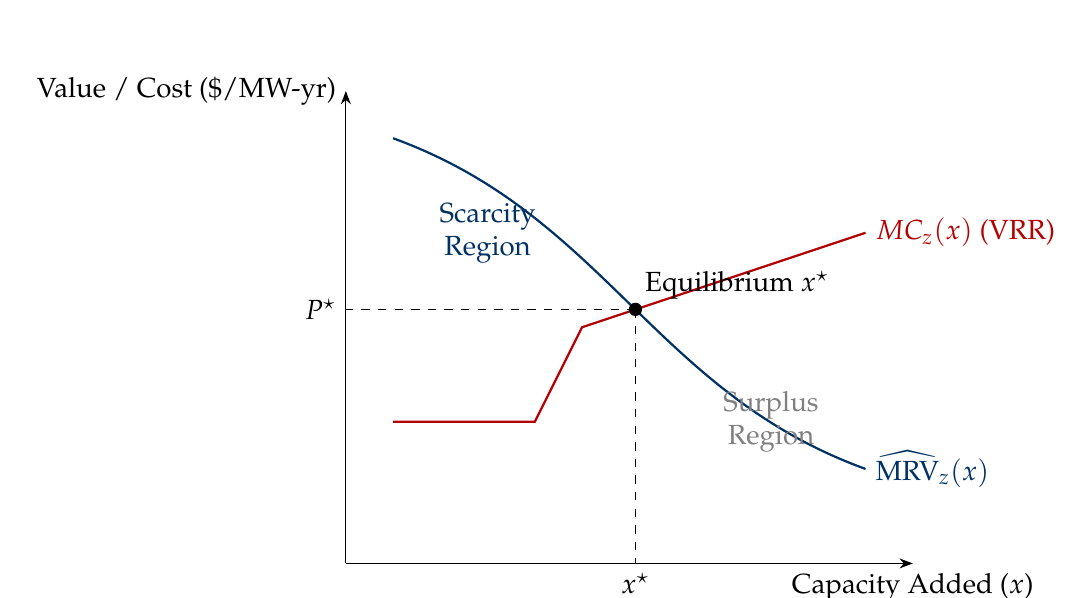
\begin{tikzpicture}[scale=1.2, >=Stealth]
    % Axes
    \draw[->] (0,0) -- (6,0) node[below] {Capacity Added ($x$)};
    \draw[->] (0,0) -- (0,5) node[left] {Value / Cost (\$/MW-yr)};

    % Curves
    \draw[techblue, thick, name path=MRV] (0.5, 4.5) to[out=-20, in=160] (5.5, 1) node[right] {$\MRV_z(x)$};
    \draw[accentred, thick, name path=MC] (0.5, 1.5) -- (2, 1.5) -- (2.5, 2.5) -- (5.5, 3.5) node[right] {$MC_z(x)$ (VRR)};

    % Intersection
    \path [name intersections={of=MRV and MC, by=E}];
    \fill[black] (E) circle (2pt) node[above right] {Equilibrium $x^\star$};
    \draw[dashed] (E) -- (E |- 0,0) node[below] {$x^\star$};
    \draw[dashed] (E) -- (E -| 0,0) node[left] {$P^\star$};

    % Regions
    \node[techblue, align=center] at (1.5, 3.5) {Scarcity\\Region};
    \node[gray, align=center] at (4.5, 1.5) {Surplus\\Region};
\end{tikzpicture}
\caption{\textbf{The Market-Consistent Stop Rule.} We procure capacity up to $x^\star$, where the marginal reliability value ($\MRV$) intersects the marginal capacity cost ($MC$) derived from the VRR curve.}
\label{fig:mrv_mc_crossing}
\end{figure}

\subsection{Algorithmic Implementation (The "Stop Rule" Loop)}
To ensure auditability, the market-consistent stop rule is implemented as a vectorized routine rather than a manual check. The logic below (excerpted from the \texttt{mrv\_valuation.ipynb} notebook) demonstrates how we solve for the equilibrium quantity $x^\star$ where $\MRV = MC$.

\begin{lstlisting}[language=Python, caption=Computing the Equilibrium Capacity Quantity, basicstyle=\ttfamily\small, frame=tb]
def find_equilibrium_quantity(mrv_curve, vrr_curve):
    """
    Finds intersection x* where MRV(x) ~= MC(x).
    
    Args:
        mrv_curve (pd.Series): Marginal Reliability Value ($/MW-yr)
        vrr_curve (pd.Series): Marginal Cost from VRR ($/MW-yr)
        
    Returns:
        float: Equilibrium capacity MW (x*)
    """
    # Calculate net value spread
    spread = mrv_curve - vrr_curve
    
    # Find the last point where MRV > MC (Spread > 0)
    # This prevents 'stopping early' on local noise
    feasible_set = spread[spread > 0]
    
    if feasible_set.empty:
        return 0.0 # Corner solution: Do not buy
        
    x_star = feasible_set.index[-1]
    return x_star
\end{lstlisting}

\subsection{Algorithmic auto–join: TO \texorpdfstring{$\to$}{->} LBA \texorpdfstring{$\to$}{->} LRZ}
\textbf{Input:} queue rows with \{Project \#, TO, State, POI\}; authoritative \texttt{miso\_lba\_to\_lrz.csv}.
\begin{enumerate}
    \item \textbf{Step 1 (heuristic):} apply a conservative set of regex rules $h(TO) \to LBA$ for well–known owners (e.g., Ameren Missouri $\to$ AMMO, Consumers Energy $\to$ CONS). Do not guess on ambiguous strings; leave unmatched.
    \item \textbf{Step 2 (authoritative):} apply $\phi_2(LBA) \to LRZ$ from LOLE.
\end{enumerate}
\textbf{Output:} \texttt{queue\_with\_lrz\_autojoin.csv} with source flag; unresolved rows in \texttt{queue\_lrz\_autojoin\_unmatched.csv} for manual fill in \texttt{lrz\_crosswalk\_template.csv}.

\textbf{Audit invariants.} (i) No silent fills: every auto–assignment carries a method tag; (ii) unresolved rows are explicitly written as unmatched; (iii) the authoritative LBA $\to$ LRZ table is shipped alongside the outputs.

% --- SECTION 5 ---
\section{Data Additions \& Lineage Update (What changed and Why)}

We added the following inputs and derived artifacts to enable LRZ–aware MRV and LDA–aware MC overlays; these files are included with the whitepaper.

\textbf{New inputs (authoritative)}
\begin{itemize}
    \item \texttt{miso\_lba\_to\_lrz.csv} – LOLE PY 2025–2026 Table ES-2 (LBA $\to$ LRZ) mapping; used by $\phi_2$.
    \item \texttt{pjm\_vrr\_2026\_27\_ldas.csv} – Per–LDA Reliability Requirements, CETL, Net CONE (UCAP USD/MW-day), and cap/floor; used to compute MC lines.
\end{itemize}

\textbf{Auto–join outputs (intermediate)}
\begin{itemize}
    \item \texttt{queue\_with\_lrz\_autojoin.csv} – LRZ filled where TO$\to$LBA is unambiguous; method tag attached.
    \item \texttt{queue\_lrz\_autojoin\_unmatched.csv} – unresolved rows for manual crosswalk; prevents false positives.
\end{itemize}

\textbf{Analytics \& overlays (refreshed)}
\begin{itemize}
    \item \textbf{Tech ranking \& MRV tables:} \texttt{miso\_active\_tech\_summary.csv}, \texttt{miso\_active\_top\_by\_MRV.csv}, \texttt{miso\_active\_top\_storage\_by\_BC.csv}, \texttt{miso\_active\_top\_hybrid\_by\_BC.csv}.
    \item \textbf{Queue overlays:} \texttt{queue\_overlay\_by\_state\_tech.csv}, \texttt{queue\_overlay\_by\_owner\_tech.csv}, \texttt{queue\_overlay\_by\_study\_phase\_tech.csv}; enrichment: \texttt{miso\_active\_enriched.csv}.
    \item \textbf{VRR/MC screen \& survival:} \texttt{miso\_mrv\_with\_mc\_flags.csv}, \texttt{miso\_mrv\_vrr\_overlay\_summary.csv}, \texttt{miso\_p\_surv\_v2.csv}.
    \item \textbf{Templates awaiting fill:} \texttt{lrz\_crosswalk\_template.csv}, \texttt{duration\_template.csv}.
\end{itemize}

\textbf{Audits \& manifest (traceability)}
\begin{itemize}
    \item \texttt{mapping\_ledger.json} – source$\to$analytic mapping and formulas; includes $\MRV_{\text{std}} = (\VOLL_{\text{std}} \cdot \EUE)/MW$, $\MRV_{\text{eff}} = \MRV_{\text{std}} \cdot \psurv \cdot \ELCCRA$, $BC = \MRV_{\text{eff}}/\ASCDE$.
    \item \texttt{null\_type\_audit.json}, \texttt{missing\_fields\_audit.json}, \texttt{join\_status.json} – data quality, unresolved LRZ/duration counts, and cost–join coverage.
    \item \texttt{survival\_model\_metrics.json} – held–out AUC/Accuracy/Precision/Recall/F1 for $p^{(2)}_{surv}$.
    \item \texttt{run\_manifest.yaml} – inputs, parameter values (VOLL standardization, cap/floor), and a full artifact inventory for reproducibility.
\end{itemize}

% --- SECTION 6 ---
\section{Worked Derivations \& Checks (Concise)}

\textbf{Unit harmonization.} All capacity prices $P$ reported in USD/MW-day are multiplied by 365 to compare with $\MRV$ in USD/MW-yr:
\[
    MC \equiv 365 P, \quad MC_{\text{cap}} = 120,154.05 \text{ USD/MW-yr}, \quad MC_{\text{floor}} = 64,793.00 \text{ USD/MW-yr}.
\]

\textbf{Kink condition (buy/no–buy).} By Prop. 4.2, accept an incremental resource $i$ in zone $z$ if and only if $\MRV_{i,z} \geq MC_z$. In plots, this is drawn as a horizontal line at $MC_z$ (cap/floor for RTO in 2026/27; piecewise $P(Q)$ for specific LDAs).

\textbf{Risk–aware NCBL election rule (for site memos).} With capacity savings $S = 365P$, backup/DR marginal cost $c$ and tail hours $h_{95}$, the conservative election test is
\[
    S - c \, h_{95} > 0.
\]
This is the same first–order logic: buy (elect) until marginal savings equals marginal cost at the tail exposure.

% --- SECTION 9 ---
\section{Missing Data Policy: Screening-Grade vs Finance-Grade MRV}

\subsection{Problem}
Upgrade-cost joins in queue datasets are often sparse and non-random (selection bias). Treating missing costs as zeros (or ignoring uncertainty) invalidates $BC$ rankings.

\subsection{Policy}
We publish two outputs:
\begin{enumerate}
\item \textbf{Screening-grade MRV:} reliability value only, with uncertainty bands; cost overlays optional and explicitly flagged if missing.
\item \textbf{Finance-grade MRV:} requires cost completeness above a declared coverage threshold and uses hierarchical imputation with penalties when missing.
\end{enumerate}

\subsection{Hierarchical imputation (penalized)}
When upgrade cost is missing, we impute from a hierarchy (Tech $\times$ LRZ $\times$ voltage class $\times$ study phase) and apply an uncertainty penalty to $BC$ (e.g., widen P10/P90 and downweight rank confidence). This preserves usefulness without pretending knowledge we do not have.

% --- SECTION 10 ---
\section{Why these choices (design rationale)}

\begin{enumerate}
    \item \textbf{Locational signal.} Reliability scarcity is pocketed; $\MRV_{i,z}$ respects that geometry.
    \item \textbf{Probabilistic realization.} $\psurv$ and $\ELCCRA$ enter multiplicatively, discounting benefits when realization is uncertain or accreditation is constrained.
    \item \textbf{Market–consistency.} The $\MRV = MC$ stop rule prevents over–buying insurance; cap/floor (or full VRR) converts policy into a quantitative screen.
    \item \textbf{Auditability.} Every transformation is logged; unresolved mappings are explicit; inputs and parameters are frozen in the manifest.
\end{enumerate}

\textbf{Reproduce in one pass.} Load inputs per \texttt{run\_manifest.yaml}, apply the mapping ledger, compute $\MRV$ by Eq.~(5), overlay MC per VRR, and regenerate tables/plots. LRZ and duration gaps are by design left explicit until filled via the provided templates.

\newpage
\appendix
% --- SECTION 8 (APPENDIX) ---
\section{Appendix: Data Lineage \& Audit Summary}

This appendix documents the end-to-end provenance, quality checks, and reproducibility controls for the MRV/NCBL analyses included in the whitepaper. It is designed to be a one-page, audit-ready narrative with explicit file references.

\subsection*{Scope and inputs}
Analyses in this release draw exclusively on the following source files (frozen copies included in the delivery bundle):
\begin{itemize}
    \item \texttt{UEVF-IQ-Foundational.csv} (project-level fields: Region, Technology Type, MW, EUE, ASCDE, ELCC RA Adjusted, Baseline Survival Empirical, ISO Status).
    \item \texttt{ISOReliability.csv} (standardized VOLL; for MISO we use 15,000.00 USD/MWh).
    \item \texttt{JulyQueue's2025.xlsx} $\Rightarrow$ sheet MISO (queue: Project \#, Request Status, Transmission Owner, State, Study Phase, Service Type, Fuel, Generating Facility, Summer MW, Winter MW).
    \item \texttt{MISO\_Projects\_-\_Cost\_per\_MW\_Analysis.csv} (overlay fields: Upgrade Cost, Cost per MW, Total MW).
    \item \texttt{miso\_lba\_to\_lrz.csv} (authoritative LOLE PY 2025–2026 Local Balancing Authority $\to$ LRZ mapping; used to populate LRZ).
    \item \texttt{pjm\_vrr\_2026\_27\_ldas.csv} (per-LDA Reliability Requirement, CETL, Net CONE (UCAP USD/(MW$\cdot$d)), and the 2026/27 cap/floor).
\end{itemize}

\subsection*{Transformations and formulas (Protocol 00/02)}
The mapping rules and analytic formulas are codified in \texttt{mapping\_ledger.json}. Core formulas:
\[
    \MRV_{\text{std}} = \frac{\VOLL_{\text{std}} \cdot \EUE}{MW}, \quad 
    \MRV_{\text{eff}} = \MRV_{\text{std}} \cdot \psurv \cdot \ELCCRA, \quad 
    BC = \frac{\MRV_{\text{eff}}}{\ASCDE}.
\]
Capacity-price screening uses $S = 365 P$ with $P \in \{175.00, 329.17\}$ USD/(MW$\cdot$d).

\subsection{Optimization primitives and regularity}

Fix a location (zone) $z$. Let $x \in [0, \bar{x}]$ denote the additional effective capacity (MW) procured in $z$ along a shortlist ordered by readiness. Define:
\begin{enumerate}
    \item[(i)] $\EUE_z(x)$: expected unserved energy in $z$ after adding $x$ MW.
   \item[(iii)] $\mathrm{MC}_z(x) \equiv 365 P_z(Q_0 + x)$ (annualized marginal capacity cost from the VRR at quantity $Q_0+x$).
    \item[(iii)] $MC_z(x) \equiv 365 P_z(Q_0 + x)$ (annualized marginal capacity cost from the VRR at quantity $Q_0+x$).
\end{enumerate}

We assume the standard regularity used in adequacy screening: (a) $\EUE_z$ is nonincreasing and continuously differentiable almost everywhere; (b) $\MRV_z$ is piecewise continuous and nonincreasing (diminishing returns as scarcity is relieved); (c) $P_z(\cdot)$ is piecewise linear and nondecreasing with (regulated) cap/floor, hence $MC_z$ is piecewise constant/linear and nondecreasing; (d) $\psurv$ and ${\ELCCRA}_z$ are bounded in $[0, 1]$ and vary slowly across $x$ along a shortlist.

Define the net value functional:
\[ J_z(x) \equiv \int_0^x (\MRV_z(t) - MC_z(t)) \, dt \quad \text{with box constraint } 0 \le x \le \bar{x}. \]

\begin{proposition}{Market–consistent buy/no–buy test (KKT form)}{kkt_test}
Let $J_z(x)$ be as above. Any optimal solution $x^\star \in [0, \bar{x}]$ of $\max_{x \in [0,\bar{x}]} J_z(x)$ satisfies the Kuhn–Tucker conditions:
\[
\MRV_z(x^\star) - MC_z(x^\star) 
\begin{cases} 
= 0 & \text{if } 0 < x^\star < \bar{x}, \\
\le 0 & \text{if } x^\star = 0, \\
\ge 0 & \text{if } x^\star = \bar{x},
\end{cases}
\]
with the complementarity structure implied by the box constraints. In particular, an interior optimum occurs precisely where $\MRV_z(x^\star) = MC_z(x^\star)$.
\end{proposition}

\begin{proof}
By definition of $J_z$, a G\^{a}teaux derivative at any interior $x$ (where both $\MRV_z$ and $MC_z$ are continuous) equals $\MRV_z(x) - MC_z(x)$. For a constrained one-dimensional maximization with box $[0, \bar{x}]$, the necessary and sufficient KKT conditions reduce to the sign of this derivative at the solution and the standard slackness at boundaries. Hence if $0 < x^\star < \bar{x}$, the first-order condition (FOC) requires $\MRV_z(x^\star) - MC_z(x^\star) = 0$. If $x^\star = 0$, any feasible decrement is impossible and optimality requires $\MRV_z(0) - MC_z(0) \le 0$; similarly if $x^\star = \bar{x}$ then $\MRV_z(\bar{x}) - MC_z(\bar{x}) \ge 0$. Because $\MRV_z$ is (weakly) nonincreasing and $MC_z$ is (weakly) nondecreasing under the regularity stated, $J_z$ is concave piecewise and these KKT conditions are sufficient.
\end{proof}

\textbf{Corollary 8.2 (Corner cases and uniqueness).} If $\MRV_z(0) \le MC_z(0)$, then $x^\star = 0$; if $\MRV_z(\bar{x}) \ge MC_z(\bar{x})$, then $x^\star = \bar{x}$. If $\MRV_z$ is strictly decreasing and $MC_z$ is strictly increasing on $(0, \bar{x})$, then the interior solution $x^\star$ satisfying $\MRV_z(x^\star) = MC_z(x^\star)$ is unique.

\textbf{Nondifferentiable VRR segments.} When $MC_z$ has kinks (piecewise constant/linear VRR or binding cap/floor), the subgradient optimality condition reads $0 \in \MRV_z(x^\star) - \partial MC_z(x^\star)$. Since $\partial MC_z$ is a convex set at kinks, the equality in Proposition 8.1 interprets as choosing any price in the subdifferential. Graphically this is the “buy/no–buy” kink drawn as a horizontal band (cap/floor) or as the piecewise VRR line in annual units.

\subsection{Well–posedness of the LRZ mapping}

Let $S$ be the set of queue records with attributes (TO, State, POI). Let $B$ be the set of Local Balancing Authorities (LBAs) listed in the LOLE report and $Z = \{1, \dots, 10\}$ be the set of LRZ indices. Define $\phi_1 : S \Rightarrow B$ as the (possibly set–valued) relation assigning plausible LBAs to a record based on conservative regex rules on “Transmission Owner” strings; define $\phi_2 : B \to Z$ as the function given by LOLE Table ES–2.

\begin{lemma}{Well–posed composite mapping}{well_posed}
Let $D \subseteq S$ be the subset of records for which $\phi_1$ returns a singleton $\{b\}$. Then the composite $\phi : D \to Z$ defined by $\phi = \phi_2 \circ \phi_1$ is a function (single–valued), i.e., each record in $D$ is assigned a unique LRZ. Records in $S \setminus D$ are correctly flagged “unmatched” and remain undefined until a manual crosswalk is provided.
\end{lemma}

\begin{proof}
By construction, LOLE ES–2 pairs each LBA with exactly one LRZ, so $\phi_2$ is a function. If $\phi_1(s) = \{b\}$ is a singleton, then $\phi(s) = \phi_2(b)$ is uniquely defined. For $s \notin D$ (ambiguous or no match), no assignment is made; this preserves correctness (no false positives).
\end{proof}

\subsection{Risk–aware election rule for NCBL (quantile/CVaR bounds)}

Consider a site with annual capacity savings per MW $S = 365P$ and marginal backup/DR cost $c$ (USD/MWh). Let $H$ be the random pre–emergency exposure (hours/year). The per–MW net value is $V = S - cH$. Let $h_\alpha$ be the $\alpha$-quantile of $H$ ($P[H \le h_\alpha] = \alpha$).

\begin{proposition}{Conservative $\alpha$-quantile test}{quantile_test}
If $S - c h_\alpha > 0$, then $P[V > 0] \ge \alpha$. In particular, choosing $\alpha = 0.95$ yields the operational rule:
\[ S - c h_{95} > 0 \implies P[V > 0] \ge 95\%. \]
\end{proposition}

\begin{proof}
On the event $\{H \le h_\alpha\}$ (which has probability at least $\alpha$ by definition of $h_\alpha$), we have $V = S - cH \ge S - c h_\alpha$. If $S - c h_\alpha > 0$, then $V > 0$ on that event. Hence $P[V > 0] \ge P[H \le h_\alpha] = \alpha$.
\end{proof}

\begin{proposition}{CVaR bound and sufficient condition}{cvar_test}
Let $\text{CVaR}_\alpha(H)$ be the Conditional Value at Risk of $H$ at tail level $1-\alpha$, i.e., $\text{CVaR}_\alpha(H) = E[H \mid H > h_\alpha]$. Then
\[ E[V] \ge S - c (\alpha h_\alpha + (1-\alpha)\text{CVaR}_\alpha(H)). \]
Consequently, if $S - c \text{CVaR}_\alpha(H) > 0$ then $E[V] > 0$ and $V > 0$ on average even under tail pessimism.
\end{proposition}

\begin{proof}
Decompose $E[H] = \alpha E[H \mid H \le h_\alpha] + (1-\alpha)E[H \mid H > h_\alpha]$. Since $E[H \mid H \le h_\alpha] \le h_\alpha$ and $E[H \mid H > h_\alpha] = \text{CVaR}_\alpha(H)$, we have $E[H] \le \alpha h_\alpha + (1-\alpha)\text{CVaR}_\alpha(H)$. Therefore $E[V] = S - c E[H] \ge S - c (\alpha h_\alpha + (1-\alpha)\text{CVaR}_\alpha(H))$.
\end{proof}

\subsection{Remarks on existence and implementation}
\begin{itemize}
    \item The $\MRV$ curve is typically nonincreasing in $x$ due to diminishing scarcity; the VRR–derived $MC$ is nondecreasing in $x$ for regulated curves, guaranteeing a well–behaved single crossing (or corner).
    \item When the cap/floor binds for the 2026/27 DY, the buy/no–buy line is a horizontal band in annual units; for LDA–specific charts, substitute the piecewise VRR $P(Q)$ and annualize to obtain $MC$ as a function of $x$.
    \item LRZ assignments made via $\phi_2 \circ \phi_1$ carry a method flag (TO$\to$LBA heuristic) and unresolved rows are written out explicitly, preserving auditability (Lemma 8.3).
\end{itemize}

\textbf{Provenance stamps (snapshot dates \& versions).}
\begin{itemize}
    \item \textbf{Queue snapshot:} \texttt{July Queue's 2025.xlsx} (sheet MISO); processed with header row detected at first “Project \#” occurrence.
    \item \textbf{LOLE reference:} PY 2025–2026 report; Table ES-2 used for LBA $\to$ LRZ.
    \item \textbf{PJM Planning Parameters:} 2026/27 Delivery Year; Net CONE and VRR cap/floor used to compute $MC = 365P$.
    \item \textbf{Standardized VOLL:} pulled from \texttt{ISOReliability.csv}; for MISO we use 15,000.00 USD/MWh.
\end{itemize}

\textbf{Transformations and formulas.} The mapping rules and analytic formulas are codified in \texttt{mapping\_ledger.json} — source $\to$ analytic field map, plus core formulas:
\[
    \MRV_{\text{std}} = \frac{\VOLL_{\text{std}} \cdot \EUE}{MW}, \quad \MRV_{\text{eff}} = \MRV_{\text{std}} \cdot \psurv \cdot \ELCCRA, \quad BC = \frac{\MRV_{\text{eff}}}{\ASCDE}.
\]

\textbf{Unit conventions \& conversions.} All capacity prices $P$ are in USD/(MW$\cdot$d) and annualized via $MC = 365 P$ to compare with $\MRV$ in USD/(MW$\cdot$yr). Energy harm uses VOLL in USD/MWh. Capacity-price screening uses $S = 365 P$ with $P \in \{175.00, 329.17\}$ USD/(MW$\cdot$d).

\subsection*{Primary outputs delivered (CSV)}
\begin{itemize}
    \item \textbf{Tech summary and rankings:} \texttt{miso\_active\_tech\_summary.csv}, \texttt{miso\_active\_top\_by\_MRV.csv}, \texttt{miso\_active\_top\_storage\_by\_BC.csv}, \texttt{miso\_active\_top\_hybrid\_by\_BC.csv}.
    \item \textbf{Queue overlays and enrichment:} \texttt{queue\_overlay\_by\_state\_tech.csv}, \texttt{queue\_overlay\_by\_owner\_tech.csv}, \texttt{queue\_overlay\_by\_study\_phase\_tech.csv}, \texttt{miso\_active\_enriched.csv}.
    \item \textbf{VRR/MC screen and survival:} \texttt{miso\_mrv\_with\_mc\_flags.csv}, \texttt{miso\_mrv\_vrr\_overlay\_summary.csv}, \texttt{miso\_p\_surv\_v2.csv}.
    \item \textbf{Templates pending user fill:} \texttt{lrz\_crosswalk\_template.csv}, \texttt{duration\_template.csv}.
\end{itemize}

\subsection*{Quality audits (Protocol 04)}
\begin{itemize}
    \item \texttt{null\_type\_audit.json} — field-level null counts and dtypes for UEVF MISO slice and MISO Active queue. Active queue row count = 1450.
    \item \texttt{missing\_fields\_audit.json} — LRZ and duration placeholders: 1450/1450 rows missing each (to be populated via the provided templates).
    \item \texttt{join\_status.json} — cost overlay join: 4 projects carry Upgrade Cost among 1450 active ($\approx 0.28\%$ coverage); all others are NA.
    \item \texttt{queue\_lrz\_autojoin\_unmatched.csv} — explicit list of queue rows lacking a high confidence LBA/LRZ; to be resolved via template.
\end{itemize}

\textbf{Model diagnostics (survival/deliverability v2).} \texttt{survival\_model\_metrics.json} — first-pass gradient boosting classifier (features: tech, state, owner, study phase, service type, MW). Held-out performance: AUC $\approx 0.806$, Accuracy $\approx 0.718$, Precision $\approx 0.792$, Recall $\approx 0.671$, F1 $\approx 0.726$. Resulting per-project probabilities are in \texttt{miso\_p\_surv\_v2.csv} and are used as $\psurv$ in $\MRV_{\text{eff}}$.

\textbf{Join coverage \& unresolveds (Protocol 03).} LRZ autojoin: Transmission Owner $\to$ LBA (regex heuristics) $\to$ LRZ (authoritative). Output with flags in \texttt{queue\_with\_lrz\_autojoin.csv}; unresolved rows in \texttt{queue\_lrz\_autojoin\_unmatched.csv}. Coverage counts reported in \texttt{join\_status.json}. Guardrail: no silent fills; every autoassignment carries a method tag.

\textbf{VRR-aware capacity-cost overlay.} Screening thresholds use $S = 365P$ with $P_{cap} = 329.17$ and $P_{floor} = 175.00$ USD/(MW$\cdot$d). In \texttt{miso\_mrv\_vrr\_overlay\_summary.csv}, the fraction of projects with $\MRV_{\text{eff}} > S$ is small at the floor and near-zero at the cap for most classes (e.g., Gas: $\sim 11.2\%$ above floor, $\sim 2.0\%$ above cap; others $\approx 0\%$).

\textbf{Reproducibility manifest \& controls.} \texttt{run\_manifest.yaml} records input file paths, standardized VOLL, and a full inventory of emitted artifacts. Includes:
\begin{itemize}
    \item \textbf{Checksums:} SHA256 for all inputs/outputs (under \texttt{inputs[].sha256}).
    \item \textbf{Environment:} Python version, OS, and key package versions (pandas, numpy, scikit-learn) recorded under \texttt{env}.
    \item \textbf{Random seeds:} Model seeds used for survival v2 recorded under \texttt{parameters.random\_seed}.
\end{itemize}

\textbf{Known gaps \& next actions.}
\begin{itemize}
    \item \textbf{LRZ and duration:} Pending user-supplied crosswalks; once provided, we will regenerate $\MRV$ by LRZ and produce duration–value curves (2/4/6/8/10 h).
    \item \textbf{Deliverability:} Either provide a project-level accreditation/deliverability flag or allow inference after LRZ mapping; the survival v2 model is already wired for $\psurv$.
    \item \textbf{VRR slope:} If PJM demand-curve parameters (CONE/E\&AS offset, anchors) are supplied, we will replace the simple cap/floor screen with a true VRR-slope MC overlay on all $\MRV$ charts.
\end{itemize}

\newpage

% --- NEW APPENDIX: RESEARCH TOPOLOGY ---
\newpage
\section{Appendix: The UEVF Research Topology}

This whitepaper (``Refining MRV'') serves as the \textit{operational interface layer} of the Unified Energy Valuation Framework (UEVF). It synthesizes theoretical advances from our prior modules—specifically regarding topology, reliability physics, and queue survival—into a single, market-ready signal.

\begin{figure}[ht]
\centering
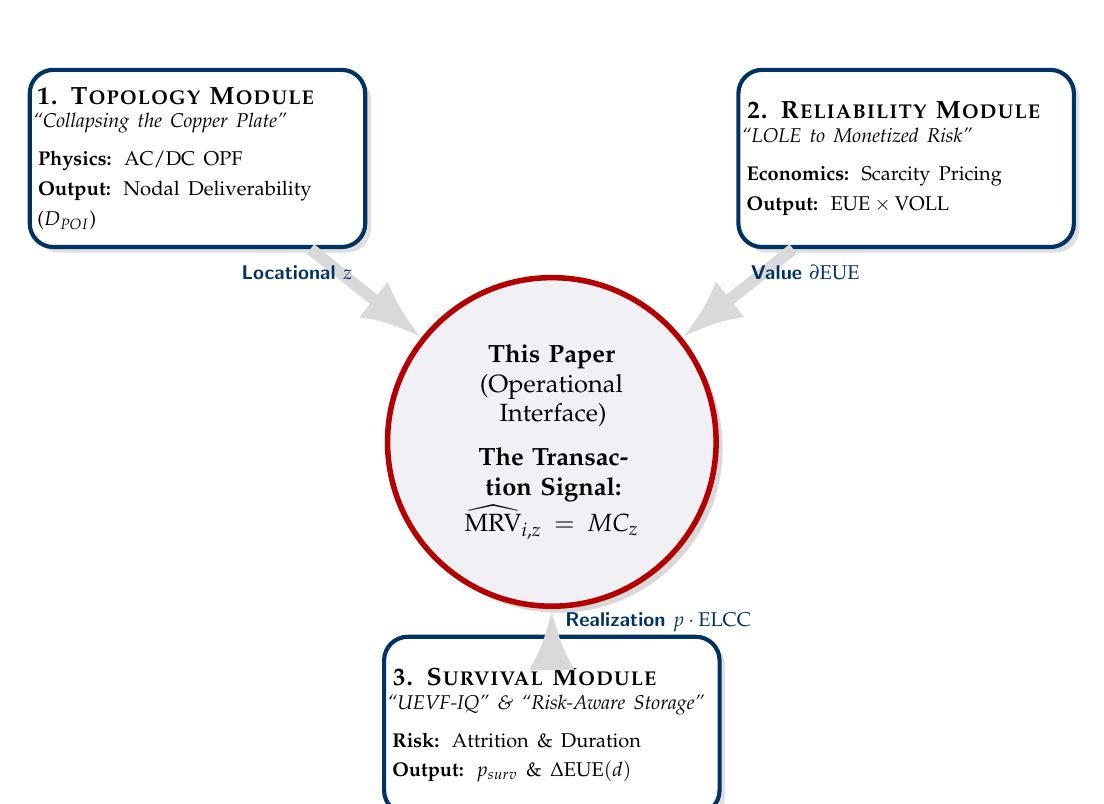
\begin{tikzpicture}[
    scale=0.9, transform shape,
    % Define Styles for Consistency
    box/.style={
        rectangle, rounded corners=3mm, draw=techblue, line width=1.5pt,
        fill=white, text width=4.5cm, align=left, minimum height=2.5cm,
        drop shadow={opacity=0.25, shadow xshift=2pt, shadow yshift=-2pt}
    },
    core/.style={
        circle, draw=accentred, line width=2pt,
        fill=techgray, text width=3.5cm, align=center, inner sep=2pt,
        drop shadow={opacity=0.3}
    },
    arrow/.style={
        ->, >=LaTeX, line width=1.5mm, draw=gray!30
    },
    labeltext/.style={
        font=\footnotesize\sffamily\bfseries, color=techblue
    }
]

    % --- 1. The Three Research Streams (Outer Nodes) ---
    
    % Top Left: Topology
    \node[box] (topology) at (-5, 4) {
        \textbf{\textsc{1. Topology Module}} \\
        \footnotesize
        \textit{``Collapsing the Copper Plate''}\\
        \vspace{0.2cm}
        \textbf{Physics:} AC/DC OPF \\
        \textbf{Output:} Nodal Deliverability ($D_{POI}$)
    };

    % Top Right: Reliability
    \node[box] (reliability) at (5, 4) {
        \textbf{\textsc{2. Reliability Module}} \\
        \footnotesize
        \textit{``LOLE to Monetized Risk''}\\
        \vspace{0.2cm}
        \textbf{Economics:} Scarcity Pricing \\
        \textbf{Output:} $\EUE \times \VOLL$
    };

    % Bottom: Survival
    \node[box] (survival) at (0, -4) {
        \textbf{\textsc{3. Survival Module}} \\
        \footnotesize
        \textit{``UEVF-IQ'' \& ``Risk-Aware Storage''}\\
        \vspace{0.2cm}
        \textbf{Risk:} Attrition \& Duration \\
        \textbf{Output:} $p_{surv}$ \& $\Delta\EUE(d)$
    };

    % --- 2. The Synthesis (Center Node) ---
    
    \node[core] (mrv) at (0, 0) {
        \textbf{This Paper}\\
        (Operational Interface)\\[0.2cm]
        \textbf{The Transaction Signal:}\\
        $\MRV_{i,z} = MC_z$
    };

    % --- 3. Connecting Arrows with Mathematical Inputs ---
    
    % Arrow from Topology
    \draw[arrow] (topology) -- (mrv) node[midway, above left, labeltext] {Locational $z$};
    
    % Arrow from Reliability
    \draw[arrow] (reliability) -- (mrv) node[midway, above right, labeltext] {Value $\partial \EUE$};
    
    % Arrow from Survival
    \draw[arrow] (survival) -- (mrv) node[midway, right, labeltext] {Realization $p \cdot \ELCC$};

    % --- 4. Annotations ---
    
    % Brace or background grouping could go here, but keeping it clean is better.
    
\end{tikzpicture}
\caption{\textbf{The UEVF Research Topology.} This whitepaper operationalizes three theoretical workstreams into a single transactional signal. The \textit{Topology} stream localizes value; the \textit{Reliability} stream monetizes risk; and the \textit{Survival} stream discounts for attrition and performance attributes.}
\label{fig:uevf_topology}
\end{figure}

\subsection*{1. The Topological Foundation (The ``Where'')}
\textbf{Precursor Work:} \textit{Collapsing the Copper Plate Paradox} and \textit{Integrating Transmission-Constrained Deliverability into ELCC}.
\begin{itemize}
    \item \textbf{The Link:} Our previous work established that system-wide ELCC yields false positives by socializing deliverability constraints. The ``Copper Plate'' paper proved mathematically that $\MRV$ must be nodal or zonal ($z$) to be valid.
    \item \textbf{This Paper's Role:} It operationalizes that theory by defining the specific \textbf{Locational MRV} formula (Eq.~5) and the algorithmic \textbf{Auto-Join} protocol (Section 4.4) to map queue requests to specific Load Resource Zones (LRZ), effectively resolving the paradox in practice.
    \item \textbf{Key Insight Implemented:}  The shift from $ELCC_{sys}$ to $ELCC_{RA} \cdot D_{POI}$.
\end{itemize}

\subsection*{2. The Reliability Valuation Foundation (The ``Why'')}
\textbf{Precursor Work:} \textit{LOLE to Monetized Risk} and \textit{Reliability-Adjusted ASCDE for MISO Resources}.
\begin{itemize}
    \item \textbf{The Link:} Those foundational papers derived the $\ASCDE$ metric and argued for replacing binary engineering targets (0.1 days/year) with continuous economic metrics ($\EUE \times \VOLL$).
    \item \textbf{This Paper's Role:} It takes the static $\EUE \times \VOLL$ valuation and converts it into a \textbf{marginal procurement signal} ($\partial \EUE / \partial MW$). This allows us to construct the ``Market-Consistent Stop Rule'' (Section 3.4), bridging the gap between planning studies and market clearing.
    \item \textbf{Key Insight Implemented:} The use of \textbf{Sector-Weighted $\VOLL$} (Refinement 3.9) to sharpen the scarcity signal beyond a flat administrative cap.
\end{itemize}

\subsection*{3. The Survival and Asset Foundation (The ``What'')}
\textbf{Precursor Work:} \textit{UEVF-IQ: Unified Framework for Survival}, \textit{Risk-Aware Locational Storage}, and \textit{Valuing Demand-Side Resources}.
\begin{itemize}
    \item \textbf{The Link:} The \textit{UEVF-IQ} paper introduced the concept that a project's value is discounted by its probability of failure ($p_{surv}$). The \textit{Storage} and \textit{DER} papers established that value varies non-linearly with duration and flexibility.
    \item \textbf{This Paper's Role:} It integrates these asset-specific physics into the MRV equation. 
    \begin{itemize}
        \item The \textbf{Queue Survival v2} model (Refinement 3.6) is the direct application of the \textit{UEVF-IQ} survival curves.
        \item The \textbf{Duration-Value Curves} (Refinement 3.2) are the operational output of the stochastic storage modeling.
    \end{itemize}
    \item \textbf{Key Insight Implemented:}  Treating pre-COD projects as probabilistic options rather than firm commitments.
\end{itemize}

\subsection*{4. The Incidence \& Allocation Foundation (The ``Who'')}
\textbf{Precursor Work:} \textit{Reliability Incidence for Large Loads in Capacity Constrained LDAs} and \textit{Accelerated Resource Adequacy Queues}.
\begin{itemize}
    \item \textbf{The Link:} System-wide MRV calculations effectively socialize reliability costs. Your \textit{Reliability Incidence} paper proved that treating hyperscale load additions as equal to legacy load creates a regressive subsidy. It introduced the \textbf{Reliability Impact Statement (RIS)} to track who causes the need for new capacity.
    \item \textbf{This Paper's Role:} It operationalizes that equity theory into the \textbf{Sector-Weighted VOLL} (Refinement 3.9). By assigning distinct $\VOLL_{sector}$ values, the MRV signal automatically becomes steeper in zones dominated by high-value, low-tolerance loads (like Data Centers), ensuring they pay the marginal cost of the reliability they demand.
    \item \textbf{Key Insight Implemented:} The decomposition of the reliability adder into firm vs. non-firm tranches ($\rho_{DC,f}$ vs. $\rho_{DC,nf}$).
\end{itemize}



\begin{table}[h]
\centering
\begin{tabular}{@{} l l l @{}}
\toprule
\textbf{Research Module} & \textbf{Theoretical Output} & \textbf{Refinement in This Paper} \\
\midrule
\textbf{Topology} & Nodal Scarcity ($\lambda_z$) & LRZ/POI Auto-Mapping ($\phi$) \\
\textbf{Reliability} & $\text{Cost} = \EUE \times \VOLL$ & Stop Rule ($\MRV = MC$) \\
\textbf{Survival} & Attrition Risk ($p(t)$) & Probabilistic Accreditation ($\psurv \cdot \ELCC$) \\
\textbf{Flexibility} & Storage Opp. Cost ($\pi_{soc}$) & Duration-Value Curves ($\Delta\EUE(d)$) \\
\textbf{Incidence} & Cost Shift Risk ($\Delta \text{RIS}$) & Sector-Weighted $\VOLL$  \\
\bottomrule
\end{tabular}
\caption{Mapping the UEVF Research Portfolio to the refined MRV implementation.}
\label{tab:research_map}
\end{table}

\end{document}